\documentclass{ctexbeamer}
\usepackage{verbatim}
\usepackage{graphicx}
\usepackage{amsmath}
\usepackage{mathtools}
\usepackage{multirow,booktabs}
\usepackage{tikz}
%\addtobeamertemplate{block begin}{%
%\setlength{\textwidth}{0.9\textwidth}%
%}{}
\usetikzlibrary{positioning}
\usetikzlibrary{calc}
\usepackage{tcolorbox}
\usepackage{empheq}
\newcommand*\widefbox[1]{\fbox{\hspace{1em}#1\hspace{1em}}}
%\usetheme{PaloAlto}
%\usetheme{CambridgeUS}
\usetheme{Berkeley}
\logo{
\includegraphics[width=1.55cm,height=1.55cm]{logo.jpg}}
\newcounter{savedenum}
\newcommand*{\saveenum}{\setcounter{savedenum}{\theenumi}}
\newcommand*{\resume}{\setcounter{enumi}{\thesavedenum}}

\begin{document}
\begin{frame}
  \title{《微波技术基础》}
  \institute{Sch.EIEE Hefei Normal University}
  \author{杨晶}
  \date{\today}
  \titlepage
\end{frame}

\begin{frame}{目录}
  \tableofcontents
\end{frame}

\begin{frame}{教材}
  《微波技术基础》,廖承恩编,西安电子科技大学出版社,2011.5.
  \begin{figure}
    \centering
    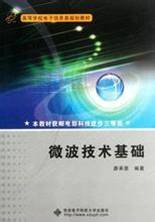
\includegraphics[height=6cm]{jiaocai}
  \end{figure}
\end{frame}

\begin{frame}{参考文献}
  \bibliographystyle{apalike}
  \nocite{Zhao}
  \nocite{Wu}
  \nocite{Colin}
  \nocite{Liang}
  \bibliography{math}
\end{frame}

\begin{frame}{考核模式}
  \begin{enumerate}
    \item 平时成绩$100$分,占总成绩$50\%$
    \begin{enumerate}
    \item 学习态度:$100$分,占$20\%$(考勤 $100$分,占$100\%$)
    \item 课堂参与:$100$分,占$30\%$(课堂表现,课堂回答问题积极性,$100$分,占$100\%$)
    \item 平时作业:$100$分,占$50\%$(书面作业$100$分,占$100\%$)
    \end{enumerate}
    \item 期末考核$100$分,占总成绩$50\%$(期末笔试$100$分,占$100\%$)
  \end{enumerate}
\end{frame}

\begin{frame}{微波技术基础}
  \begin{description}
    \item[第一章] \textcolor{red}{引论}
    \item[第二章] \textcolor{red}{传输线理论}
    \item[第三章] \textcolor{red}{规则金属波导}
    \item[第四章] \textcolor{red}{微波集成传输线}
    \item[第五章] 毫米波介质波导与光波导
    \item[第六章] \textcolor{red}{微波网络基础}
    \item[第七章] \textcolor{red}{微波谐振器}
    \item[第八章] \textcolor{red}{常用微波元件}
    \item[第九章] 微波铁氧体元件
  \end{description}
\end{frame}

\section{第一章\quad 引论}
\begin{frame}{第一章\quad 引论}
  \begin{enumerate}
    \item 微波及其特点
    \item 微波的应用
    \item 本书的内容框图
    \item 导行波及其一般的传输特性
  \end{enumerate}
\end{frame}

\begin{frame}{近代通信技术的发展}
  \begin{columns}
    \begin{column}{0.35\linewidth}
      \centering
      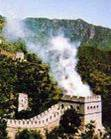
\includegraphics[height=5cm]{fenghuotai}
    \end{column}
    \begin{column}{0.65\linewidth}
      \centering
      \begin{itemize}
        \item 人类历史上最早的通信手段和现在一样是“无线”的。
        \item 人类通信史上革命性变化,是从把电作为信息载体后发生的。
      \end{itemize}
    \end{column}
  \end{columns}
\end{frame}

\begin{frame}{电报的发明}
  \begin{columns}
    \begin{column}{0.5\linewidth}
      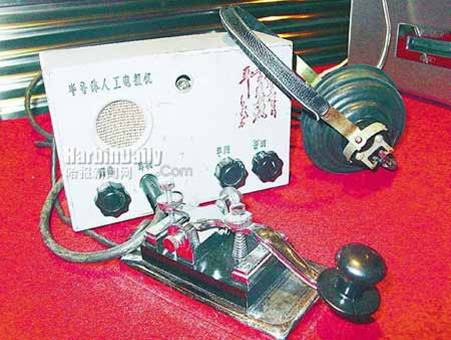
\includegraphics[height=4cm]{dianbao}
    \end{column}
    \begin{column}{0.5\linewidth}
      \begin{itemize}
        \item 电报的发明,拉开了电信时代的序幕,开创了人类利用电来传递信息的历史。
      \end{itemize}
    \end{column}
  \end{columns}
\end{frame}

\begin{frame}{电报的发明}
  \begin{columns}
    \begin{column}{0.5\linewidth}
    \begin{figure}
      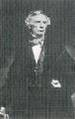
\includegraphics[width=3.5cm]{Morse.jpg}
      \caption{莫尔斯 Morse.Samrel Finley.Breese (1791-1872)}\label{Morse}
    \end{figure}
    \end{column}
    \begin{column}{0.5\linewidth}
      \begin{itemize}
        \item 美国画家莫尔斯
        \item 在1835年,第一台电报机问世
      \end{itemize}
    \end{column}
  \end{columns}
\end{frame}

\begin{frame}{电报的发明}
  \begin{itemize}
    \item 莫尔斯成功地利用电流的“通”、“断”和“长断”来代替了人类的文字进行传送,这就是鼎鼎大名的莫尔斯电码。
  \end{itemize}
  \centering
  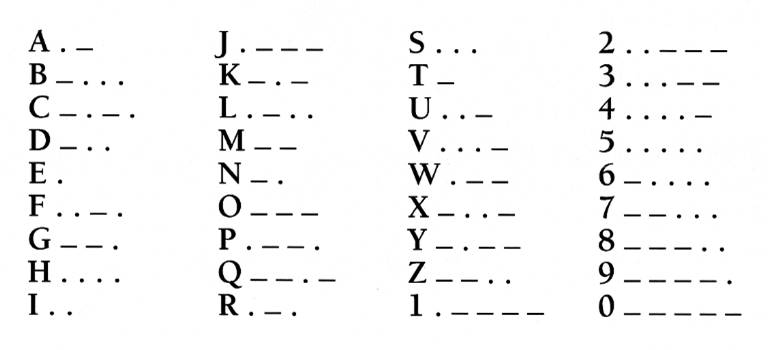
\includegraphics[width=8cm]{morsecode}
\end{frame}

\begin{frame}{电话的发明}
  \begin{columns}
    \begin{column}{0.35\linewidth}
      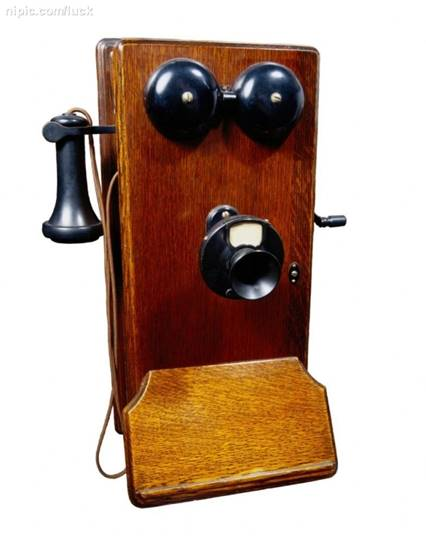
\includegraphics[height=6.5cm]{dianhua}
    \end{column}
    \begin{column}{0.65\linewidth}
      \begin{itemize}
        \item 1875年6月2日,被人们作为发明电话的伟大日子而加以纪念,而美国波士顿法院路109号也因此载入史册,至今它的门口仍钉着块铜牌,上面镌有:“1875年6月2日电话诞生在此。”
      \end{itemize}
    \end{column}
  \end{columns}
\end{frame}

\begin{frame}{电话的发明}
  \begin{columns}
    \begin{column}{0.4\linewidth}
    \begin{figure}
      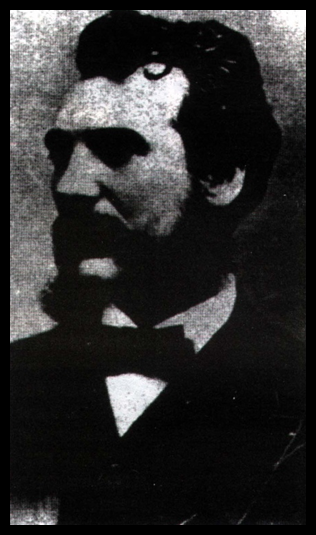
\includegraphics[width=3.2cm]{Bell.png}
      \caption{亚历山大·格拉汉姆·贝尔Alexander Graham Bell (1847 - 1922)}
    \end{figure}
    \end{column}
    \begin{column}{0.6\linewidth}
      \begin{itemize}
        \item 美国发明家和企业家。他获得了世界上第一台可用的电话机的专利权(发明者为意大利人安东尼奥·梅乌奇),创建了贝尔电话公司(AT\&T公司的前身)。其被世界誉为“电话之父”。
      \end{itemize}
    \end{column}
  \end{columns}
\end{frame}

\begin{frame}{电话的发明}
  \begin{columns}
    \begin{column}{0.5\linewidth}
      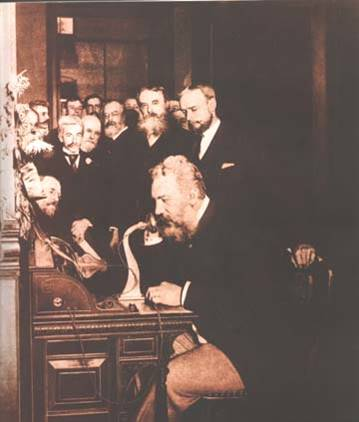
\includegraphics[width=5.5cm]{Bell2}
    \end{column}
    \begin{column}{0.5\linewidth}
      \begin{itemize}
        \item 贝尔在1892年启用第一条长途电话线——从纽约至芝加哥,长约900里。
      \end{itemize}
    \end{column}
  \end{columns}
\end{frame}

\begin{frame}{电话的发明}
  \begin{columns}
    \begin{column}{0.35\linewidth}
      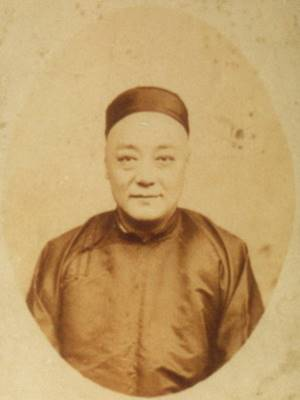
\includegraphics[width=3.5cm]{pengmingbao}
    \end{column}
    \begin{column}{0.65\linewidth}
      \begin{itemize}
        \item 电话传入我国,是在1881年,英籍电气技师皮晓浦在上海十六铺沿街架起一对露天电话,付36文制钱可通话一次,这是中国的第一部电话。1882年2月,丹麦大北电报公司在上海外滩扬于天路办起我国第一个电话局,用户25家。
        \item 1889年,安徽省安庆州候补知州\textbf{彭名保},自行设计了一部电话,包括自制的五六十种大小零件,称为我国第一部自行设计制造的电话。
      \end{itemize}
    \end{column}
  \end{columns}
\end{frame}

\begin{frame}{电磁波的发现}
  % Electromagnetic wave - black
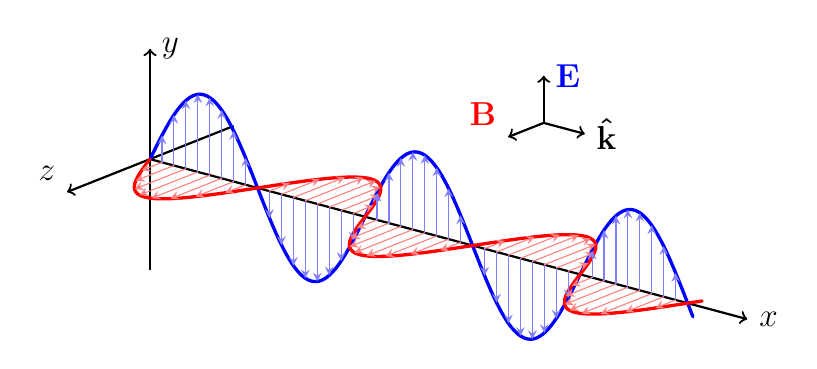
\begin{tikzpicture}[x=(-15:0.9), y=(90:1.0), z=(-150:1.0),
                    line cap=round, line join=round,
                    axis/.style={black, thick,->},
                    vector/.style={>=stealth,->}]
  \large
  \def\A{1}
  \def\nNodes{5} % use even number
  \def\nVectorsPerNode{8}
  \def\N{\nNodes*40}
  \def\xmax{\nNodes*pi/2*1.01}
  \pgfmathsetmacro\nVectors{(\nVectorsPerNode+1)*\nNodes}

  \def\vE{{\color{blue}\mathbf{E}}}
  \def\vB{{\color{red}\mathbf{B}}}
  \def\vk{\mathbf{\hat{k}}}

  % main axes
  \draw[axis] (0,0,0) -- ++(\xmax*1.1,0,0) node[right] {$x$};
  \draw[axis] (0,-\A*1.4,0) -- (0,\A*1.4,0) node[right] {$y$};
  \draw[axis] (0,0,-\A*1.4) -- (0,0,\A*1.4) node[above left] {$z$};

  % small axes
  \def\xOffset{{(\nNodes-2)*pi/2}}
  \def\yOffset{\A*1.2}
  \def\zOffset{\A*1.2}
  \draw[axis] (\xOffset,\yOffset,-\zOffset) -- ++(\A*0.6,0,0) node[right] {$\vk$};
  \draw[axis] (\xOffset,\yOffset,-\zOffset) -- ++(0,\A*0.6,0) node[right] {$\vE$};
  \draw[axis] (\xOffset,\yOffset,-\zOffset) -- ++(0,0,\A*0.6) node[above left] {$\vB$};

  % equation
  %\node[above right] at (\xOffset,-0.5*\yOffset,4*\zOffset)
  %  {$\begin{aligned}
  %    \vE &= \mathbf{E_0}\sin(\vk\cdot\mathbf{x}-c_0t)\\
  %    \vB &= \mathbf{B_0}\sin(\vk\cdot\mathbf{x}-c_0t)\\
  %    \end{aligned}$};
  %\node[below right] at (\xOffset,-0.5*\yOffset,4*\zOffset)
  %  {$\vE\cdot\vk = 0,\;\; \vB\cdot\vk = 0,\;\; \vB = \frac{1}{c_0}\vk\times\vE$};

  % waves
  \draw[blue,very thick,variable=\t,domain=0:\nNodes*pi/2*1.01,samples=\N]
    plot (\t,{\A*sin(\t*360/pi)},0);
  \draw[red,very thick,variable=\t,domain=0:\nNodes*pi/2*1.01,samples=\N]
    plot (\t,0,{\A*sin(\t*360/pi)});

  % draw vectors
  \foreach \k [evaluate={\t=\k*pi/2/(\nVectorsPerNode+1);
                         \angle=\k*90/(\nVectorsPerNode+1);
                         \c=(mod(\angle,90)!=0);}]
              in {1,...,\nVectors}{
    \if\c1
      \draw[vector,blue!50] (\t,0,0) -- ++(0,{\A*sin(2*\angle)},0);
      \draw[vector,red!50] (\t,0,0) -- ++(0,0,{\A*sin(2*\angle)});
    \fi
  }
\end{tikzpicture}
\begin{itemize}
  \item 自从贝尔发明了电话机,这样人人都能手拿一个“话柄”,和远方的亲朋好友谈天说地了。电报和电话的相继发明,使人类获得了远距离传送信息的重要手段。但是,电信号都是通过金属线传送信息的重要手段。但是,电信号都是通过金属线传送的。线路架设到的地方,信息才能传到,这就大大限制了信息的传播范围,特别是在大海、高山,有没有能让信息\textbf{无线}传播的方法?
\end{itemize}
\end{frame}

\begin{frame}{电磁波的发现}
  \begin{columns}
    \begin{column}{0.35\linewidth}
    \begin{figure}
      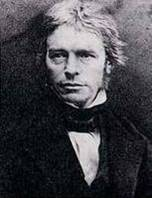
\includegraphics[width=3.5cm]{faraday.jpg}
      \caption{迈克尔·法拉第Michael Faraday(1791-1867)}
    \end{figure}
    \end{column}
    \hfill
    \begin{column}{0.65\linewidth}
      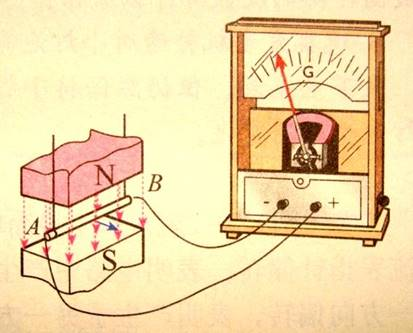
\includegraphics[width=5cm]{faradayexperiment.jpg}
      \begin{itemize}
        \item 英国物理学家、化学家
        \item 1831年发现电磁感应
      \end{itemize}
    \end{column}
  \end{columns}
\end{frame}

\begin{frame}{电磁波的发现}
  \begin{columns}
    \begin{column}{0.35\linewidth}
      \begin{figure}
        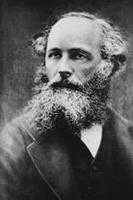
\includegraphics[width=3.5cm]{maxwell.jpg}
        \caption{詹姆斯·克拉克·麦克斯韦James Clerk Maxwell (1831-1879)}
      \end{figure}
    \end{column}
    \begin{column}{0.65\linewidth}
      Maxwell Equations:
      %\begin{equation}
        \begin{align*}
          &\nabla\times\vec E=-\frac{\partial \vec B}{\partial t}\\
          &\nabla\times\vec H=\vec{J} +\frac{\partial \vec D}{\partial t}\\
          &\nabla\cdot\vec{D}=\rho\\
          &\nabla\cdot\vec{B}=0
        \end{align*}
      %\end{equation}
      \begin{itemize}
        \item 英国物理学家。1864年,麦氏发表了电磁场理论,成为人类历史上预言电磁波存在的\textbf{第一人}
      \end{itemize}
    \end{column}
  \end{columns}
\end{frame}

\begin{frame}{电磁波的发现}
  \begin{columns}
    \begin{column}{0.35\linewidth}
      \begin{figure}
        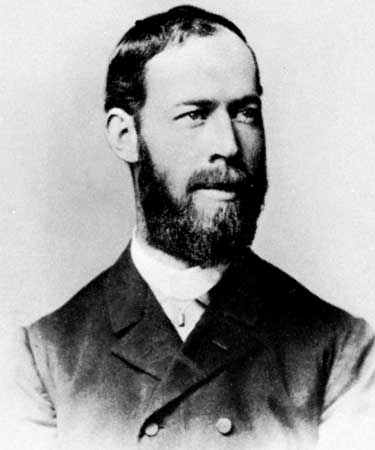
\includegraphics[width=3cm]{hertz.jpg}
        \caption{亨利希·鲁道夫·赫兹(1857 - 1894)}
      \end{figure}
    \end{column}
    \begin{column}{0.65\linewidth}
      \begin{figure}
        \flushright
        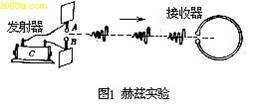
\includegraphics[width=2.5cm]{hertzexperiment.jpg}
      \end{figure}
      \begin{itemize}
        \item 德国物理学家,1887年,实验证实了电磁波的存在和传播。成为了近代科学技术史的一座里程碑,为了纪念这位杰出的科学家,电磁波的单位便命名为“赫兹($Hz$)”
        \item 证明了麦克斯韦理论的正确,导致了无线电的诞生,开辟了电子技术的新纪元,标志着从“有线电通信”向“无线电通信”的转折点。也是整个移动通信的发源点,应该说,从这时开始,人类开始进入了无线通信的新领域。
      \end{itemize}
    \end{column}
  \end{columns}
\end{frame}

\subsection{1\quad 微波及其特点}
\begin{frame}{微波及其特点}
  电磁波按波长(或频率)划分,则大致可以把$300MHz - 3000GHz$,(对应空气中波长$\lambda$是$1m - 0.1mm$)这一频段的电磁波称之为微波。它处于超短波和红外光波之间。
\end{frame}

\begin{frame}{微波波段的划分}
  \begin{tabular}{cccc}
    \toprule
    波段代号 & 标称波长/cm & 频率范围/GHz & 波长范围/cm \\
    \midrule
     L & 22 & 1-2 & 30-15 \\
     S & 10 & 2-4 & 15-7.5 \\
     C & 5 & 4-8 & 7.5-3.5 \\
     X & 3 & 8-12 & 3.75-2.5 \\
     Ku & 2 & 12-18 & 2.5-1.67 \\
     K & 1.25 & 18-27 & 1.67-1.11 \\
     Ka & 0.8 & 27-40 & 1.11-0.75 \\
     U & 0.6 & 40-60 & 0.75-0.5 \\
     V & 0.4 & 60-80 & 0.5-0.375 \\
     W & 0.3 & 80-100 & 0.375-0.3 \\
     \bottomrule
  \end{tabular}
\end{frame}

\begin{frame}{Maxwell方程组的物理意义}
  \begin{columns}
    \begin{column}{0.4\linewidth}
      \begin{align*}
        & \nabla\times\vec{E} = -\frac{\partial \vec{B}}{\partial t}\\
        & \nabla\times\vec{H} = \vec{J}+\frac{\partial \vec{D}}{\partial t}
      \end{align*}
    \end{column}
    \begin{column}{0.6\linewidth}
      \begin{itemize}
        \item 这两个方程左边物理量为磁(或电),而右边物理量则为电(或磁)。这中间的等号深刻揭示了电与磁的相互转化,相互依赖,相互对立,共存于统一的电磁波中。正是由于电不断转换为磁,而磁又不断转换成为电,才会发生能量交换和贮存。
      \end{itemize}
    \end{column}
  \end{columns}
\end{frame}

\begin{frame}{电与磁的转换}
  \begin{itemize}
    \item Oersted和Faraday的实验证实了电磁转换,而且还知道了只有动磁才能转化为电。
    \item 还需提到:电磁转换为电磁波的出现提供了可能,但不一定是现实。例如电磁振荡也是典型的电磁转换,但没有引起\textbf{波(Wave)}。
    \item 作为力学类比,电磁转换犹如单摆问题中的动能与势能的转化。
  \end{itemize}
\end{frame}

\begin{frame}{Maxwell方程组的物理意义}
  \begin{itemize}
    \item 进一步研究Maxwell方程两边的运算,从物理上看,运算反映一种作用(Action)。方程左边是空间运算(\textbf{旋度});方程右边是时间运算(\textbf{导数}),中间用等号连接。它深刻揭示了电(或磁)场任一地点的变化会转化为磁(或电)场时间的变化;反过来,场的时间变化也会转化成地点的变化。正是这种空间和时间的相互变化构成了波动的外在形式。用通俗的一句话说:即\textbf{一个地点出现过的事物,过了一段时间又在另一地点出现了}。
  \end{itemize}
\end{frame}

\begin{frame}{Maxwell方程组的物理意义}
  \begin{columns}
    \begin{column}{0.4\linewidth}
      \begin{align*}
        & \nabla\times\vec{H} = j\omega\epsilon\vec{E}+\vec{J}\\
        & \nabla\times\vec{E} = -j\omega\mu\vec{H}
      \end{align*}
    \end{column}
    \begin{column}{0.6\linewidth}
      \textbf{单色波}频域的$Maxwell$方程
    \end{column}
  \end{columns}
\begin{itemize}
  \item $Maxwell$方程还指出:电磁转化有一个重要条件,即频率$\omega$。只有较高的$\omega$才能确保电磁的有效转换,直流情况没有转换。可以这样说,在高频封闭电路才有可能变成开放电路。不过很有意思的是频率越高,越难输出功率,这也是一个有趣的矛盾。
\end{itemize}
\end{frame}

\begin{frame}{Maxwell方程组的物理意义}
  \begin{columns}
    \begin{column}{0.4\linewidth}
      \begin{align*}
        &\nabla\times\vec E=-\frac{\partial \vec B}{\partial t}\\
        &\nabla\times\vec H=\vec{J} +\frac{\partial \vec D}{\partial t}\\
        &\nabla\cdot\vec{D}=\rho\\
        &\nabla\cdot\vec{B}=0
      \end{align*}
    \end{column}
    \begin{column}{0.65\linewidth}
      \begin{itemize}
        \item 在Maxwell方程中还存在另一对矛盾对抗,这就构成了Maxwell方程本质的不对称性。尽管为了找其对称性而一直在探索磁流$\vec{M}$的存在,但到目前为止始终未果。
      \end{itemize}
    \end{column}
  \end{columns}
\end{frame}

\begin{frame}{微波的特点}
  \begin{enumerate}
    \item 微波的两重性\\ 微波的两重性指的是对于尺寸大的物体,如大型建筑物、山谷等它显示出粒子的特点——即似光性或直线性,而对于相对尺寸小的物体,又显示出——波动性或似声性。
    \item 微波与“左邻右舍”的比较\\ 微波的“左邻”是超短波和短波,而它的“右舍”又是红外光波。
    \saveenum
  \end{enumerate}
  \begin{columns}
    \begin{column}{0.44\linewidth}
      \begin{tcolorbox}[colback=blue!5,colframe=blue!40!black,title=微波与超短波、短波比较]
        微波与超短波、短波相比较大大扩展了通讯通道,开辟了微波通讯和卫星通讯。
      \end{tcolorbox}
    \end{column}
    \begin{column}{0.55\linewidth}
      \begin{tcolorbox}[colback=blue!5,colframe=blue!40!black,title=微波与光波比较]
        微波与光波比较,光通过雨雾衰减很大,特别是雾天,蓝光、紫光几乎看不见,这正是采用红光作警戒的原因。而微波波段穿透力强。
      \end{tcolorbox}
    \end{column}
  \end{columns}
\end{frame}

\begin{frame}{微波的特点}
  \begin{enumerate}
    \resume
    \item 宇宙“窗口”\\地球的外层空间由于日光等繁复的原因形成独特的电离层,它对于短波几乎全反射,这就是短波的天波通讯方式。因而在微波波段则有若干个可以通过电离层的“宇宙窗口”。因而微波是独特的宇宙通讯手段。
    \saveenum
  \end{enumerate}
  \centering
  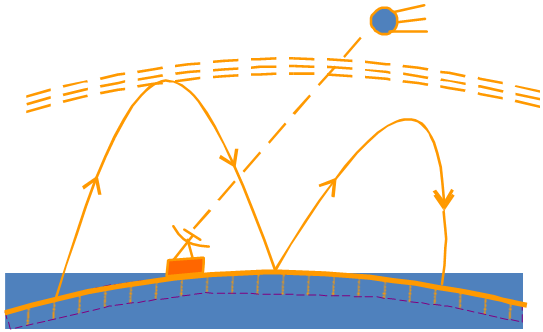
\includegraphics[width=6.5cm]{cosmicwindow.png}
\end{frame}

\begin{frame}{微波的特点}
  \begin{enumerate}
    \resume
    \item 计算机的运算次数进入十亿次,其频率也是微波频率。超高速集成电路的互耦也是微波互耦问题,因此,微波的研究已进入集成电路和计算机。
    \item 微波研究方法主要有两种:场论的研究方法和网络的研究方法。这也是本门课程要学习的重要方法。其中场论方法的基础是本征模理论。网络方法的基础是广义传输线理论。
  \end{enumerate}
\end{frame}

\subsection{2\quad 微波的应用}
\begin{frame}{微波技术的应用}
  \begin{tikzpicture}
    \node[draw,
    %fill=blue,
    minimum width=2cm,
    minimum height=1.2cm]
    (sum) at (0,0){微波应用};
  \end{tikzpicture}
\end{frame}

\begin{frame}{微波技术的发展}

\end{frame}

\subsection{3\quad 本课程内容}
\begin{frame}{本课程内容}
  \begin{columns}
    \begin{column}{0.15\linewidth}
      \begin{enumerate}
        \item 引论
        \saveenum
      \end{enumerate}
    \end{column}
    \begin{column}{0.35\linewidth}
      \textcolor{blue}{均匀传输线和波导理论基础}\\
      \textcolor{blue}{微波电路元件}
    \end{column}
    \begin{column}{0.5\linewidth}
      \begin{enumerate}
        \resume
        \item \textbf{传输线理论}
        \item \textbf{规则金属波导}
        \item \textbf{微波集成电路}
        \item 毫米波介质波导与光波导
        \item \textbf{微波网络基础}
        \item \textbf{微波谐振器}
        \item \textbf{常用微波器件}
        \item 微波铁氧体元件
      \end{enumerate}
    \end{column}
  \end{columns}
\end{frame}

\begin{frame}{微波技术的研究方法}

\end{frame}

\subsection{4\quad 导行波及其传输特性}
\begin{frame}{基本概念}
  \begin{enumerate}
    \item \textbf{导行系统(Guided system)}
    \saveenum
    \\约束或导引电磁能量定向传播\\
    作用:\\
    \begin{itemize}
      \item 无辐射损耗的将电磁波从一处传到另一处
      \item 设计成微波元件:滤波器、阻抗变换器、定向耦合器等。
    \end{itemize}
    微波电路是一种由各种导行系统构成的导行电磁波电路
  \end{enumerate}

\end{frame}

\begin{frame}{导行系统结构}
  %\begin{figure}
    \centering
    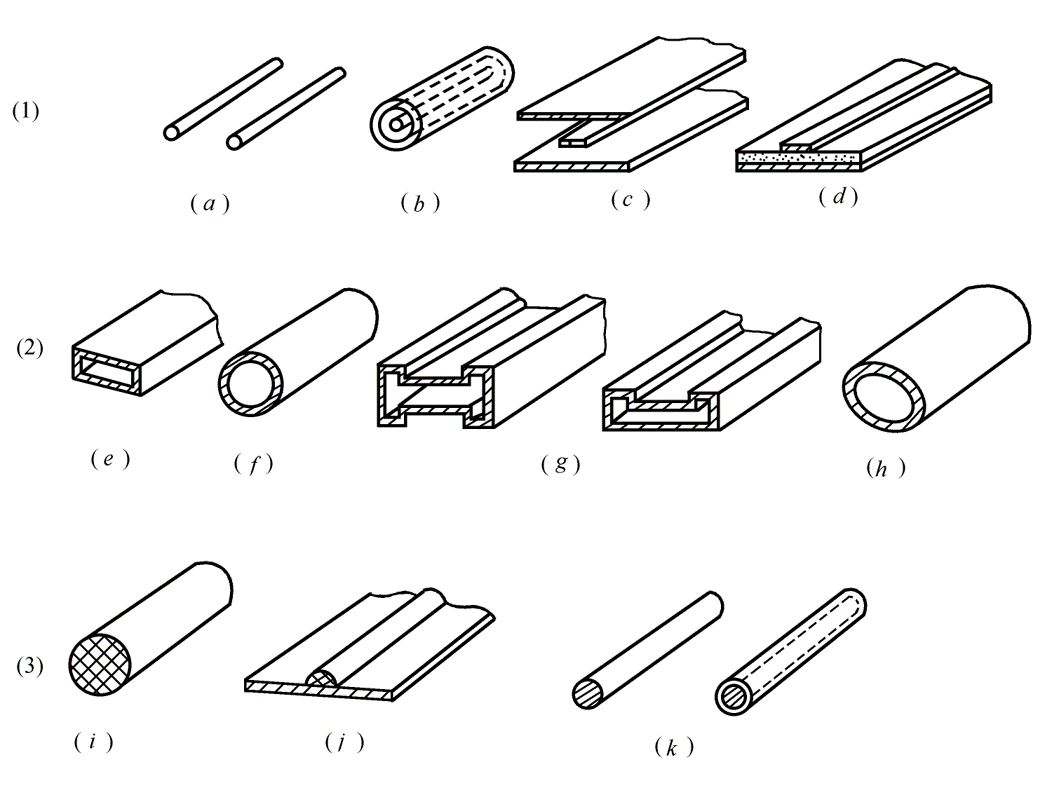
\includegraphics[width=9cm]{guidesystem.png}
  %\end{figure}
\end{frame}

\begin{frame}{基本概念}
  \begin{enumerate}
    \resume
    \item \textbf{导行波(Guided Wave)}
    \\沿导行系统定向传播的电磁波(导波)
    \\\textbf{TEM波}\quad 横电磁波 —— 各种传输线 电磁能量约束或限制在导体之间的空间内沿其轴向传播
    \\\textbf{TE/TM波}\quad 横电/横磁波 —— 封闭金属波导 电磁能量完全限制在金属管内沿轴向传播
    \\\textbf{表面波} —— 开波导 电磁能量约束在波导结构的周围(波导内和波导表面附近)沿轴向传播
    \saveenum
  \end{enumerate}
\end{frame}

\begin{frame}{基本概念}
  \begin{enumerate}
    \resume
    \item \textbf{导模(Guided mode)}
    \\导行波的模式(传输模)
    \\ *在导行系统横截面上的电磁场呈驻波分布,且完全确定的,与位置和频率无关
    \\ *导模是离散的,当频率一定时,每个导模具有唯一的传播常数
    \\ *导模之间相互正交,彼此独立,互不耦合
    \\ *具有截止特性,截止条件和截止波长因导行系统和模式而异
    \item \textbf{规则导行系统(Regular guided system)}
    \\无限长笔直导行系统,其横截面尺寸、媒质分布、结构材料、边界条件沿轴向均不变化
  \end{enumerate}
\end{frame}

\begin{frame}{导波场的分析}
  在\textbf{均匀}、\textbf{无耗}、\textbf{各向同性}、\textbf{无源}导行系统中
  \begin{columns}
    \begin{column}{0.5\linewidth}
      \begin{empheq}[box=\widefbox]{align*}
        &\nabla\times\vec E=-\frac{\partial \vec B}{\partial t}\\
        &\nabla\times\vec H=\vec{J} +\frac{\partial \vec D}{\partial t}\\
        &\nabla\cdot\vec{D}=\rho\\
        &\nabla\cdot\vec{B}=0
      \end{empheq}
      设导波沿$z$向传播,坐标$z$与横向坐标无关
    \end{column}
    \begin{column}{0.5\linewidth}
      \flushright
      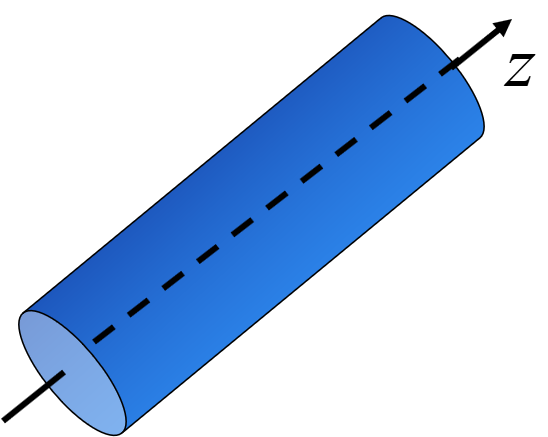
\includegraphics[width=4cm]{zuobiao.png}
      \begin{align*}
        & \nabla=\nabla_{t}+\hat z \partial / \partial z\\
        & \vec E=\vec E_{t}+\hat z E_{z}\\
        & \vec H=\vec H_{t}+\hat z H_{z}
      \end{align*}
    \end{column}
  \end{columns}
\end{frame}

\newcommand{\mtikzmark}[1]{\tikz[overlay,remember picture]\node(#1){};}
\tikzset{mylabel/.style={align=center,fill=blue!10,font=\footnotesize}}
%\mytlabel[options]{start.mark}{end.mark}{text}
\newcommand\mytlabel[4][]{%
\tikz[overlay,remember picture]
{\draw[->]([yshift=-10pt]#2.north) -- node[mylabel,#1]{#4}([yshift=6pt]#3.north);}
}
\begin{frame}{导波场的分析}
  \begin{columns}
    \begin{column}{0.45\linewidth}
      \begin{empheq}[box=\widefbox]{align*}
        %\tikzmarkin{c}(0.05,-0.6)(-0.05,0.65)
        & \nabla_t\times\vec{H_{t}}=j\omega\epsilon\hat{z}E_{z} \\
        & \nabla_t\times\hat{z}H_{z}+\hat{z}\times\frac{\partial\vec{H_{t}}}{\partial z}
        = \mtikzmark{a}j\omega\epsilon\vec{E_{t}}
      \end{empheq}
      %$$\times j\omega\mu$$
    \end{column}
    \begin{column}{0.5\linewidth}
      \begin{empheq}[box=\widefbox]{align*}
        & \nabla_t\times\vec E_{t}=-j\omega\mu\hat{z} H_{z} \\
        & \nabla_t\times \hat z E_{z}+\hat{z}\times\mtikzmark{c}\frac{\partial\vec{E_{t}}}{\partial z}
        = -j\omega\mu\vec{H_t}
      \end{empheq}
    \end{column}
  \end{columns}
  \begin{flalign*}
      & j\omega\mu\hat{z}\times\frac{\partial \vec{H_{t}}}{\partial z}=\mtikzmark{b}-j\omega\mu\nabla_{t}\times\hat{z}H_{z}-\omega^{2}\mu\epsilon\vec{E_{t}} &
  \end{flalign*}
  \begin{flalign*}
    && -j\omega\mu\hat{z}\times\frac{\partial \vec{H_{t}}}{\partial z}=\hat{z}\times\frac{\partial}{\partial z} \left(\nabla_{t}\times\hat{z}E_{z}\right)+\hat{z}\times\mtikzmark{d}\frac{\partial}{\partial z} \left(\hat{z} \times \frac{\partial \vec{E_{t}}}{\partial z} \right)
  \end{flalign*}
  % draw arrow with text from specified position to another
  \mytlabel{a}{b}{$\times j\omega\mu$}
  \mytlabel{c}{d}{$\hat{z}\times\frac{\partial}{\partial z}$}
\end{frame}

\begin{frame}{导波场的分析}
  \begin{empheq}[box=\widefbox]{align*}
    \left( k^{2}+\frac{\partial^{2}}{\partial z^{2}} \right)\vec{E_{t}}=\frac{\partial}{\partial z}\nabla_{t}E_{z}-j\omega\mu\nabla_{t}\times\hat{z}H_{z}
  \end{empheq}
  \begin{empheq}[box=\widefbox]{align*}
    \left( k^{2}+\frac{\partial^{2}}{\partial z^{2}} \right)\vec{H_{t}}=\frac{\partial}{\partial z}\nabla_{t}H_{z}-j\omega\epsilon\nabla_{t}\times\hat{z}E_{z}
  \end{empheq}
  在规则导行系统中,导波场的\textbf{横向分量}可用\textbf{纵向分量}完全确定。\\上面公式中$k^{2}=\omega^{2}\mu\epsilon$
\end{frame}

\begin{frame}{导波场的分析}
  \begin{empheq}[box=\widefbox]{align*}
    & \nabla^{2}\vec{E}+k^{2}\vec{E}=0\\
    & \nabla^{2}\vec{H}+\mtikzmark{a}k^{2}\vec{H}=0
  \end{empheq}
  \begin{columns}
    \begin{column}{0.45\linewidth}
      \begin{empheq}[box=\widefbox]{align*}
        & \nabla^{2}E_{z}+\mtikzmark{b}k^{2}E_{z}=0\\
        & \nabla^{2}H_{z}+\mtikzmark{d}k^{2}H_{z}=0
      \end{empheq}
    \end{column}
    \begin{column}{0.45\linewidth}
      \begin{empheq}[box=\widefbox]{align*}
        & \nabla^{2}\vec{E}_{t}+\mtikzmark{c}k^{2}\vec{E}_{t}=0\\
        & \nabla^{2}\vec{H}_{t}+k^{2}\vec{H}_{t}=0
      \end{empheq}
    \end{column}
  \end{columns}
  \flushright
  \begin{empheq}[box=\widefbox]{align*}
    \left( \nabla^{2}_{t}+\frac{\partial^{2}}{\partial z^{2}}\right)
    \left\{\begin{aligned}
      \mtikzmark{e}E_{z}(z,t)\\H_{z}(z,t)
    \end{aligned}\right\}
    +k^{2}
    \left\{\begin{aligned}
      E_{z}(z,t)\\H_{z}(z,t)
    \end{aligned}\right\}
    =0
  \end{empheq}
  \mytlabel{a}{b}{纵向场}
  \mytlabel{a}{c}{横向场}
  \mytlabel{d}{e}{Helmholtz Equation}
\end{frame}

\begin{frame}{导波场的分析}
  \begin{empheq}[box=\widefbox]{align*}
    \left( \nabla^{2}_{t}+\frac{\partial^{2}}{\partial z^{2}}\right)
    \left\{\begin{aligned}
      \mtikzmark{e}E_{z}(z,t)\\H_{z}(z,t)
    \end{aligned}\right\}
    +k^{2}
    \left\{\begin{aligned}
      E_{z}(z,t)\\H_{z}(z,t)
    \end{aligned}\right\}
    =0
  \end{empheq}
  \begin{enumerate}
    \item \textbf{分离变量法}\\
    令$E_{z}(z,t)=Z(z)E_{0z}(t)$ \\
    \begin{align*}
      \frac{\nabla_{t}^{2}E_{0z}(t)}{E_{0z}(t)}+\frac{d^{2}Z(z)/dz^{2}}{Z(z)}=-k^{2}
    \end{align*}
    \begin{columns}
      \begin{column}{0.3\linewidth}
        分离变量常数: $k_{c}$和$\beta$
      \end{column}
      \begin{column}{0.6\linewidth}
        \begin{empheq}[box=\widefbox]{align*}
          & d^{2}Z(z)/dz^{2}+\beta^{2}Z(z)=0 \\
          & \nabla_{t}^{2}E_{0z}(t)+k_{c}^{2}E_{0z}(t)=0
        \end{empheq}
        \flushright————本征值方程
      \end{column}
    \end{columns}
    \saveenum
  \end{enumerate}
\end{frame}

\begin{frame}{导波场的分析}
  \begin{enumerate}
    \resume
    \item \textbf{色散关系}
    \begin{columns}
      \begin{column}{0.55\linewidth}
        \begin{empheq}[box=\widefbox]{align*}
          & k^{2}=k_{c}^{2}+\beta^{2}\\
          & \beta=\sqrt{k^{2}-k_{c}^{2}}=k\sqrt{1-(k_{c}/k)^{2}}
        \end{empheq}
      \end{column}
      \begin{column}{0.4\linewidth}
        \raggedright
        $k^{2}=\omega^{2}\mu\epsilon$\\  $\beta$:导波的传播常数或相移常数
      \end{column}
    \end{columns}
    $$d^{2}Z(z)/dz^{2}+\beta^{2}Z(z)=0$$
    %\flushleft
    解:
    \begin{empheq}[box=\widefbox]{align*}
      Z(z)=A_{1}exp(-j\beta z)+A_{2}exp(j\beta z)
    \end{empheq}
    \textbf{规则导行系统中沿正$z$方向传播的导波纵向场分量}\\
    \begin{align*}
      E_{z}(t,z)=E_{0z}(t)exp(-j\beta z)\\
      H_{z}(t,z)=H_{0z}(t)exp(-j\beta z)
    \end{align*}
    \saveenum
  \end{enumerate}
\end{frame}

\begin{frame}{导波场的分析}
  \begin{enumerate}
    \resume
    \item 本征值方程
    \begin{empheq}[box=\widefbox]{align*}
      \nabla_{t}^{2}E_{0z}(t)+k_{c}^{2}E_{0z}(t)=0
    \end{empheq}
    $k_{c}$:在特定边界条件下的本征值,称为导波的横向截止波数\\
    $k_{c}\neq 0$
    \saveenum
  \end{enumerate}
\end{frame}

\begin{frame}{导波场的分析}
  \begin{enumerate}
    \resume
    \item 横-纵向场的关系
    \begin{empheq}[box=\widefbox]{align*}
      \left( k^{2}+\frac{\partial_{2}}{\partial z^{2}}\right)\vec{E}_{t}=\frac{\partial}{\partial z}\nabla_{t}E_{z}-j\omega\mu\nabla_{t}\times\hat{z}H_{z}\\
      \left( k^{2}+\frac{\partial_{2}}{\partial z^{2}}\right)\vec{H}_{t}=\frac{\partial}{\partial z}\nabla_{t}H_{z}-j\omega\epsilon\nabla_{t}\times\hat{z}E_{z}
    \end{empheq}
    \begin{columns}
      \begin{column}{0.6\linewidth}
        \begin{empheq}[box=\widefbox]{align*}
          \vec{E}_{t}=\frac{-j\beta}{k_{c}^{2}}\left[\nabla_{t}E_{z}+Z_{h}\nabla_{t}H_{z}\times\hat{z}\right]\\
          \vec{H}_{t}=\frac{-j\beta}{k_{c}^{2}}\left[\nabla_{t}H_{z}+Y_{e}\hat{z}\times\nabla_{t}E_{z}\right]
        \end{empheq}
      \end{column}
      \begin{column}{0.4\linewidth}
        \begin{align*}
          Z_{h}=\sqrt{\frac{\mu}{\epsilon}}\frac{k}{\beta}\\
          Y_{e}=\sqrt{\frac{\epsilon}{\mu}}\frac{k}{\beta}
        \end{align*}
      \end{column}
    \end{columns}
    \saveenum
  \end{enumerate}
\end{frame}

\begin{frame}{导波场的分析}
  \begin{enumerate}
    \resume
    \item 导波的种类\\
    \begin{block}{横磁波(TM)或电(E)波——$H_{z}=0$}
      \begin{empheq}[box=\widefbox]{align*}
        \vec{E}_{t}^{e}=\frac{-j\beta}{k_{c}^{2}}\nabla_{t}E_{z}\qquad
        \vec{H}_{t}^{e}=\frac{-j\beta}{k_{c}^{2}}Y_{e}\hat{z}\times\nabla_{t}E_{z}
      \end{empheq}
    \end{block}
    \begin{block}{横电波(TE)或磁(H)波——$E_{z}=0$}
      \begin{empheq}[box=\widefbox]{align*}
        \vec{E}_{t}^{h}=\frac{-j\beta}{k_{c}^{2}}Z_{h}\nabla_{t}H_{z}\times\hat{z}\qquad
        \vec{H}_{t}^{h}=\frac{-j\beta}{k_{c}^{2}}\nabla_{t}H_{z}
      \end{empheq}
    \end{block}
    导行系统横向为调谐(振动)解形式$k_{c}^{2}>0$,$k^{2}>\beta^{2}$;$\beta=k\cdot\sqrt{1-\left(\frac{k_{c}}{k}\right)^{2}}$ 相速$v_{p}>c/\sqrt{\epsilon_{r}}$快波,有色散性,且需满足$k_{c}<k$才能传播。
  \end{enumerate}
\end{frame}

\begin{frame}{导波场的分析}
  \begin{block}{横电磁波(TEM)——$E_{z}=H_{z}=0$}
    %\begin{flalign*}
      $$ \because E_{t}\neq 0,H_{t}\neq 0 $$
    %\end{flalign*}
    以及
    \begin{align*}
      & \vec{E}_{t}=\frac{-j\beta}{k_{c}^{2}}[\nabla_{t}E_{z}+Z_{h}\nabla_{t}H_{z}\times\hat{z}]\\
      & \vec{H}_{t}=\frac{-j\beta}{k_{c}^{2}}[\nabla_{t}H_{z}+Y_{e}\hat{z}\times\nabla_{t}E_{z}]
    \end{align*}
    $$\left(\frac{0}{0}\right)\text{形式}\Longrightarrow k_{c}=0 \qquad k^{2}=k_{c}^{2}+\beta^{2}\Longrightarrow \beta=k $$
  \end{block}
\end{frame}

\begin{frame}{导波场的分析}
  又由$\nabla_{t}\times\vec{E}_{t}=-j\omega\mu\hat{z}H_{z}$\qquad$\nabla_{t}\times\vec{H}_{t}=j\omega\epsilon\hat{z}E_{z}$
  \begin{empheq}[box=\widefbox]{align*}
    \nabla_{t}\times\vec{E}_{t}^{0}=0 \qquad \nabla_{t}\times\vec{H}_{t}^{0}=0
  \end{empheq}
  $$\nabla_{t}\times\hat{z}E_{z}+\hat{z}\times\frac{\partial\vec{E}_{t}}{\partial z}=-j\omega\mu\vec{H}_{t} \qquad \nabla_{t}\times\hat{z}H_{z}+\hat{z}\times\frac{\partial\vec{H}_{t}}{\partial z}=j\omega\epsilon\vec{E}_{t} $$
  \begin{columns}
    \begin{column}{0.2\linewidth}
      \begin{empheq}[box=\widefbox]{align*}
        & \frac{\partial}{\partial z}=-j\beta \\ & k=\omega\sqrt(\mu\epsilon)
      \end{empheq}
    \end{column}
    \begin{column}{0.75\linewidth}
      \begin{empheq}[box=\widefbox]{align*}
        \vec{E}_{t}^{0}\times \hat{z}=-\eta\vec{H}_{t}^{0} \qquad \eta\vec{H}_{t}^{0}\times\hat{z}=\vec{E}_{t}^{0}\quad \text{TEM波}
      \end{empheq}
    \end{column}
  \end{columns}
  \begin{columns}
    \begin{column}{0.4\linewidth}
      固有阻抗$\eta=\sqrt(\mu/\epsilon)\text{且}$
    \end{column}
    \begin{column}{0.5\linewidth}
      \begin{empheq}[box=\widefbox]{align*}
        \nabla_{t}^{2}\vec{E}_{0t}^{0}(t)=0 \quad \nabla_{t}^{2}\vec{H}_{0t}^{0}(t)=0
      \end{empheq}
    \end{column}
  \end{columns}
  TEM的导波场与静态场相同,存在于导体之间,或由双导体或多导体构成的导行系统(传输线)中,故又称为传输线模式;导波的相速、群速与无耗媒质平面波相同,无色散现象。
\end{frame}

\begin{frame}{导波场的分析}
  混合波\quad——\quad\fbox{$k_{c}^{2}<0$}\\导行系统横向为衰减解形式,场被束缚在导行系统表面——表面波可存在于电抗壁导行系统中,例如:介质波导、光纤等。
  \begin{empheq}[box=\widefbox]{align*}
    k^{2}<\beta^{2}\rightarrow v_{p}<c/\sqrt{\epsilon_{r}}
  \end{empheq}
  \textbf{称为慢波,且需满足$k_{c}<k$才能传播}
\end{frame}

\begin{frame}{导行波的一般传输特性}
  \begin{enumerate}
    \item \textbf{导模的截止波长与传输条件}\\
    导行系统中某导模无衰减能传播的最大波长——\textbf{截止波长}$\lambda_{c}$ \\
    导行系统中某导模无衰减能传播的最小频率——\textbf{截止频率}$f_{c}$ \\
    导波的传播常数\quad \widefbox{$\beta=k\sqrt{1-(k_{c}/k)^{2}}$} \\
    为虚数时,导模不能传播。\\
    当$k^{2}=\omega^{2}\mu\epsilon=k_{c}^{2}$时$\beta=0$,导模截止。\\
    对应的截止频率\quad$\Longrightarrow$\quad $\omega\sqrt{\mu\epsilon}=k_{c}$ \\
    截止频率:\widefbox{$f_{c}=\frac{k_{c}}{2\pi\sqrt{\mu\epsilon}}$}\\
    截止波长:\widefbox{$\lambda_{c}=\frac{2\pi}{k_{c}}$}
    \saveenum
  \end{enumerate}
\end{frame}

\begin{frame}{导行波的一般传输特性}

\end{frame}

\begin{frame}{导行波的一般传输特性}

\end{frame}

\begin{frame}{导行波的一般传输特性}

\end{frame}

\end{document}
